\subsection{Solver Algorithmen} \label{sec:solver}
 
\subsubsection[Dimensionsbestimmung]{Dimensionsbestimmung \myAuthor{Luis Schubert}} \label{sec:matrix_size_calculation}
Da zunächst die Dimensionen des Puzzles nicht bekannt, diese jedoch zum Lösen der Puzzles hilfreich sind, können sie wie folgt bestimmt werden.
Um die Anzahl der Zeilen $r$ und Spalten $c$ aus der Anzahl der Puzzleteile $p$ und Kanten $k$ zu berechnen dient folgendes Gleichungssystem:
\begin{align*}
    g_1 :=& p = r \cdot c \\
    g_2 :=& k = 2(c + r) - 4 ~~.
\end{align*}
Auflösen nach $r$ und $c$ ergibt
\begin{align*}
    c =& \frac{ 2 + \frac{1}{2}k + \sqrt{(4 + 2 k + \frac{1}{4}k^2 - 4 p)}}{2} \text{ und}\\
    r =& \frac{p}{c} ~~.
\end{align*}



\subsubsection[Tiefensuche]{Tiefensuche \myAuthor{Jonas Leitner}} \label{sec:depth_search}
Nachdem durch den Extractor \ref{sec:extractor} und den Matcher \ref{sec:matcher} die Grundlagen für die Repräsentation von Puzzleteilen sowie für die Erhebung von Ähnlichkeitswerten zwischen einzelnen Kanten geschaffen wurden, ist es nun möglich, einen darauf aufbauenden Algorithmus zu entwickeln, der das Puzzle lösen kann.

Ein erster primitiver Gedanke war, die Matrix Position für Position mittels einer Tiefensuche (Depth Search) zu durchlaufen und jeweils das Puzzleteil auszuwählen, das am besten zum vorherigen passt. 
Dies ist jedoch schwierig, solange man die genaue Größe des Puzzles nicht kennt. 
Aus diesem Grund war eine weitere Idee, wie wir Menschen es auch oft tun, zuerst den gesamten Rahmen des Puzzles zu konstruieren.

\paragraph{Frame Builder}
Konzentriert man sich zunächst nur auf ein Teilproblem, ist dieses leichter zu lösen. Für den Puzzle-Rahmen müssen nur noch CORNER- und EDGE-Pieces betrachtet werden. Auch Validierungen, ob ein Puzzleteil mit einer bestimmten Rotation an eine Stelle passt, sind wesentlich einfacher zu handhaben. 
% Durch die Berechnung der Puzzlegröße (siehe \autoref{sec:matrix_size_calculation}) 

Aus diesem Grund wurde der $FrameBuilder$ entwickelt, dessen Aufgabe darin besteht, den kompletten Rahmen des Puzzles aufzubauen. Der Algorithmus versucht, den Rahmen im Uhrzeigersinn aufzubauen, bis keine CORNER- oder EDGE-Pieces mehr vorhanden sind und somit der Rahmen geschlossen ist.
Der Ablaufplan des gesamten Algorithmus ist in \autoref{fig:frame_builder} dargestellt.

\begin{figure}[ht] 
    \centering 
    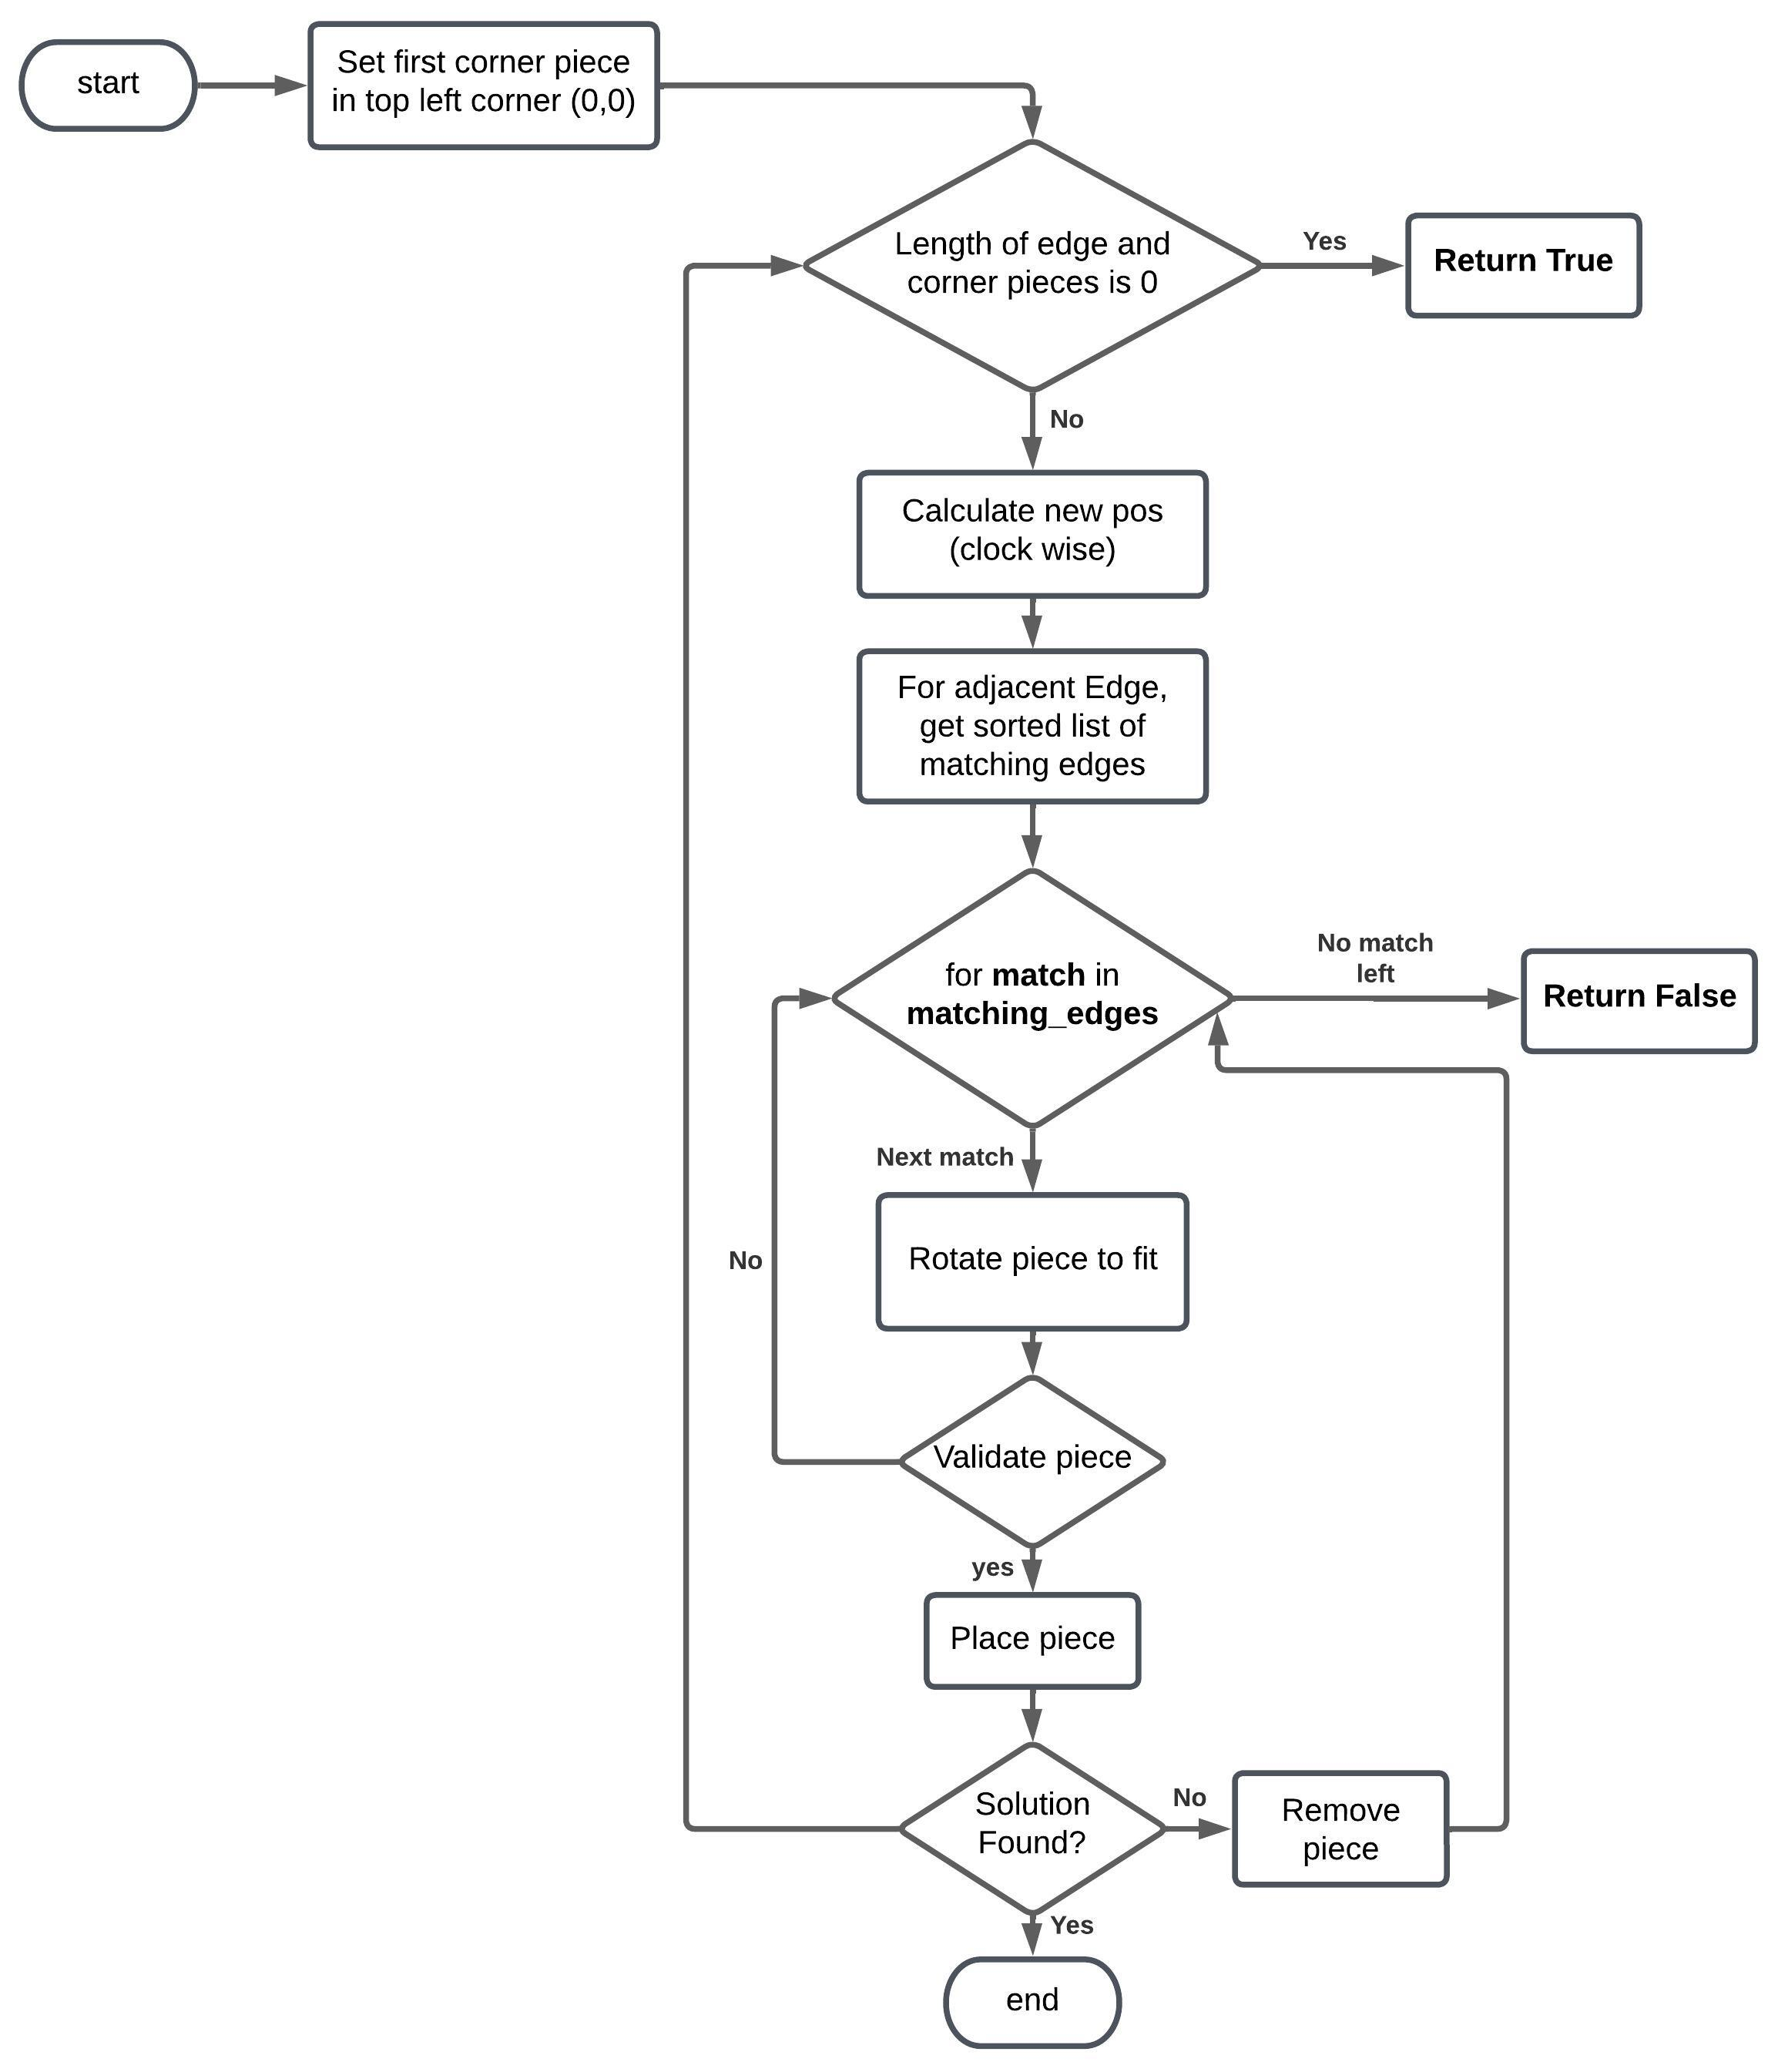
\includegraphics[width=0.8\textwidth]{images/frame_builder.jpeg} 
    \caption{Frame Builder Algorithmus} 
    \label{fig:frame_builder} 
    \end{figure}    

Zur Initiierung wird eines der vier Eckpuzzleteile in die obere linke Ecke positioniert. Im Anschluss beginnt der rekursive Teil des Algorithmus.
In jedem Schritt wird das zuvor platzierte Puzzleteil mit seiner Position sowie einer sogenannten Build Direction übergeben.
Der Algorithmus beginnt mit der Prüfung der Abbruchbedingung, bei der festgestellt wird, ob noch EDGE- oder CORNER-Puzzleteile zum Platzieren vorhanden sind.
Im Anschluss erfolgt die Berechnung der nächsten Position. Die nachfolgende Position ist dabei abhängig vom vorherigen Puzzleteil sowie der sogenannten Build Direction. 

\begin{itemize}
    \item Im Falle eines EDGE-Puzzleteils wird die Build Direction beibehalten.
Wird also nach rechts gebaut, dann ist die neue Position $x = x + 1, y = y$.
    \item Wohingegen, wenn das vorherige Puzzleteil eine Ecke war, dann wird die Build Direction gewechselt. Handelt es sich um die zweite Ecke, dann ändert sich die Build Direction von rechts nach unten. Bei der dritten von unten zu links und so weiter.
\end{itemize}

In einem nächsten Schritt wird für die anliegende $Edge$, eine Liste an Matching Edges vom $Matcher$ erstellt. Diese ist sortiert, wobei die am besten passende Kante zuerst kommt.
In einer Schleife, die mit dem besten Match beginnt, wird nun das zur Edge dazugehörige Puzzleteil geladen und in die korrekte Position rotiert. Danach wird mit dem zugrundeliegenden Wissen validiert, ob das Puzzleteil auch an die Stelle passt.

Durch die Build Direction weis man automatisch an welcher Stelle die FLAT-Edge platziert sein muss. Diese muss stets nach außen zeigen. Zudem weis man durch die Berechnung der Puzzlegröße (siehe \autoref{sec:matrix_size_calculation}), an welchen Positionen ein CORNER-Piece kommen muss. Schlägt die Validierung fehl, wird der nächstbeste Match probiert. Andernfalls wird das PuzzlePiece platziert und die Funktion erneut rekursiv aufgerufen. 
Wurden alle möglichen Matches ausprobiert, jedoch konnte keine erfolgreiche Piece-Platzierung gefunden werden, wird eine Rekursionsstufe höher gegangen und das zuvor platzierte Puzzleteil entfernt. 
Anschließend wird auf der Ebene das nächstbeste Puzzleteil probiert. Dieser Prozess wird solange wiederholt, bis entweder erfolgreich alle EDGE- und CORNER-Pieces platziert wurden und somit eine Lösung gefunden wurde oder bis alle möglichen Optionen ausprobiert wurden und keine Lösung gefunden werden konnte.

\paragraph{Lösen des Puzzles-Inneren}

Im nächsten Schritt kann das Innere des Puzzles gelöst werden. Da der Puzzlerahmen die Dimension des Puzzles vorgibt, kann nun Reihe für Reihe durchgegangen werden. 
Der Algorithmus startet an Position $(1,1)$. Wie im $FrameBuilder$ wird der Algorithmus wieder Schritt für Schritt rekursiv aufgerufen. Zu Beginn wird die Abbruchbedingung geprüft, indem festgestellt wird, ob das Puzzle noch $available\_pieces$ zum Setzen hat.

\begin{algorithm}[H]
\caption{Depth-Search-Algorithmus}\label{alg:depth_search_algorithm}
\begin{algorithmic}[1]
\State \textbf{Eingabe:} Puzzle mit gelöstem Rahmen
\State \textbf{Ausgabe:} gelöstes Puzzle
\State $start\_pos \gets$ (1,1)
\State \Call{next\_piece}{$start\_pos$}
\State \Comment{Rekursive Funktion für jedes weitere Puzzleteil}
\Function{next\_piece}{$pos$}
    \State $available\_pieces \gets$ puzzle.available\_pieces
    \If {len($available\_pieces$) == 0} \Comment{Abbruchbedingung}
        \State \Return True
    \EndIf
    \State $adjacent\_edges \gets$ puzzle.get\_adjacent\_edges($pos$)
    \State $matching\_pieces \gets$ matcher.get\_matching\_pieces($adjacent\_edges$)
    
    \For{$matching\_piece  \in matching\_pieces$}
        \State \texttt{Rotiere} $matching\_piece$
        \State \texttt{Platziere} $matching\_piece$ an $pos$
        
        \State $new\_pos \gets$ get\_next\_position($pos$) \Comment{Berechnet Position Reihe für Reihe}

        \If{\Call{next\_piece}{$new\_pos$}}
            \State \Return True
        \Else
            \State \texttt{Entferne} $matching\_piece$ an $pos$
        \EndIf      
    \EndFor
    
\EndFunction
\end{algorithmic}
\end{algorithm}

Ein Vorteil gegenüber der vorherigen Situation im $FrameBuilder$ ist zudem, dass sich an einer Position nun immer mindestens zwei anliegende Kanten befinden. Über die $Puzzle$-Klasse kann für eine bestimmte Position die Menge aller $adjacent\_edges$ abgefragt werden. Mithilfe dieser kann über die $Matcher$-Funktion $get\_matching\_pieces()$ die Menge aller passenden Puzzleteile berechnet werden, die wie folgt funktioniert:

Für jede Edge in den angrenzenden $n$ Edges wird eine Liste von Matches erzeugt. Aus dieser wird jeweils aus der EdgeID die PieceID zurückgerechnet: $PieceID = EdgeID \div 4$. Über alle $n$ Listen wird dann die Schnittmenge gebildet. 
Dies ist notwendig, da die passenden Edges auch alle zum selben Puzzleteil gehören müssen. In einem weiteren Schritt werden dann die übrig gebliebenen Pieces für die Position in allen vier Rotierungsvarianten getestet: 
\begin{enumerate}
    \item Dabei wird zunächst festgestellt, ob die passenden Edges auch an den passenden Positionen liegen. Im Falle, dass die $adjacent\_edges$ beispielsweise oben und links sind, müssen die passenden Edges am Piece auch in der selben Reihenfolge nebeneinander liegen.
    \item Des Weiteren kann ein Piece auch in mehreren Rotierungen an die Position passen.
    \item Für jede mögliche Position wird zudem der passende Match Score durch Aufsummieren der einzelnen Edge Scores berechnet.
\end{enumerate}
 Die Liste der Matching Pieces wird nach Score absteigend sortiert.

In einer Schleife wird nun wieder mit dem am besten passenden Match begonnen. Das Puzzleteil wird in die entsprechende Position rotiert und platziert. Im Anschluss erfolgt die Berechnung der nächsten Position, welche von links nach rechts Reihe für Reihe durchgegangen wird. Im nächsten Schritt wird eine Rekursionsstufe weitergegangen. Falls auf einer Ebene wiederum alle Matches ausprobiert wurden oder keine passenden Matches gefunden wurden, wird in der Ebene höher das letzte Puzzleteil entfernt.
Dieser Prozess wird wiederholt, bis eine Lösung gefunden wurde oder alle Optionen ausprobiert wurden.

\subsubsection[Best-First-Algorithmus]{Best-First-Algorithmus \myAuthor{Jonas Leitner}}
Ist die Qualität der Vergleichswerte für die Edges gut, so lässt sich bereits eine hohe Effektivität des Depth-Search-Algorithmus feststellen. 
Wählt der Algorithmus jedoch gleich zu Beginn ein „falsches” Puzzleteil aus, sucht er sehr tief nach der richtigen Lösung, die er nie finden kann. Er müsste im Grunde den gesamten Suchbaum aufwärts gehen, um zu einem anderen Zweig zu gelangen. Dieser Prozess kann sehr ineffizient sein und viel Zeit in Anspruch nehmen.

Aus diesem Grund wurde ein weiterer Lösungsansatz entwickelt, der eine breitere Suche nach dem bestmöglichen Match ermöglicht.
Anstatt nur für eine bestimmte Position den besten Match zu ermitteln, können alle offen liegenden Edges berücksichtigt werden. Genau diesen Ansatz verfolgt der Best-First-Algorithmus (siehe Algorithmus \ref{alg:best_first_algorithm}).

\begin{algorithm}[H]
\caption{Best-First-Algorithmus}\label{alg:best_first_algorithm}
\begin{algorithmic}[1]
\State \textbf{Eingabe:} Puzzle mit gelöstem Rahmen
\State \textbf{Ausgabe:} gelöstes Puzzle
\State $exposed\_edges \gets$ Initialisiere mit $puzzle$ \Comment{Alle inneren Kanten des Rahmens}
\State \Call{next\_piece}{$exposed\_edges$}
\State \Comment{Rekursive Funktion für jedes weitere Puzzleteil}
\Function{next\_piece}{$exposed\_edges$}
    \State $\text{available\_pieces} \gets$ puzzle.available\_pieces
    \If {len($available\_pieces$) == 0} \Comment{Abbruchbedingung}
        \State \Return True
    \EndIf

    \State $exposed\_edge\_scores \gets$ get\_exposed\_edge\_scores()
    \State $adjacent\_pos\_scores \gets$  get\_best\_adjacent\_pos($exposed\_edge\_scores$)

    \For{$\text{pos} \in \text{adjacent\_pos\_scores}$}
        \State $adjacent\_edges \gets$ puzzle.get\_adjacent\_edges($pos$)
        \State $matching\_piece \gets$ matcher.get\_matching\_pieces($adjacent\_edges$)[0]
        \State \texttt{Rotiere} $matching\_piece$
        \State \texttt{Platziere} $matching\_piece$ an $pos$

        \State $updated\_exposed\_edges \gets$ Aktualisiere $exposed\_edges$ Liste

        \If{\Call{next\_piece}{$updated\_exposed\_edges$}}
            \State \Return True
        \Else
            \State \texttt{Entferne} $matching\_piece$ an $pos$
        \EndIf      
    \EndFor
    
\EndFunction
\end{algorithmic}
\end{algorithm}

Zu Beginn erfolgt die Initialisierung der offen liegenden Kanten (exposed\_edges). Dies umfasst alle nach innen gerichteten Kanten des bereits erstellten Rahmens. Im Vergleich zum Depth-Search-Algorithmus wird nun nicht mehr eine Position in die Rekursionsfunktion gegeben, sondern eine Liste an exposed\_edges. Im Anschluss muss für alle offen liegenden Kanten jeweils der bestmögliche Matchscore ermittelt werden. Diese werden in $exposed\_edge\_scores$ gespeichert.

Die Match Scores könnten bereits sortiert und mit dem höchsten Match begonnen werden. Es besteht jedoch die Möglichkeit, einen weiteren Schritt einzubauen, wenn davon ausgegangen wird, dass ein Match besser ist, sobald mehrere Edges an einer Position anliegen.
Für alle Exposed Edges kann geschaut werden, an welcher Position sie anliegen, der Score der Position ergibt sich durch die anliegenden Edges. Gibt es mehrere Edges, wird der Score summiert. 
Genau dieser Schritt wird durch die Funktion $get\_best\_adjacent\_pos()$ ausgeführt. 

Der Algorithmus beginnt mit der besten Position und berechnet für diese wie im Depth-Search-Algorithmus das beste $matching\_piece$. Dieses wird rotiert und platziert. Im nächsten Schritt muss die Liste der Exposed Edges aktualisiert werden. Dazu werden die zuvorigen Exposed Edges, die an der platzierten Position waren, entfernt und die durch das neue Puzzle Piece hinzugekommenen Exposed Edges hinzugefügt. 
Ansonsten ist die Funktionsweise des Algorithmus identisch mit der des Depth-First-Algorithmus.

\paragraph{Easy-First Ansatz}
Die Algorithmen sind abhängig von den Vergleichswerten, die der Matcher liefert. In Fällen, in denen die Werte zwischen den einzelnen Matches sehr nah aneinander sind, könnte dies für den Best-First-Algorithmus zu Schwierigkeiten führen.
Eine Modifikation stellt der Easy-First-Algorithmus dar. Alternativ zur Festlegung des Scores lediglich am besten Match kann bei der Funktion $get\_exposed\_edge\_scores()$ auch die Differenz zum nächsten Match als Score verwendet werden:
$$
    score_{eid} = matches[0] - matches[1]
$$

Hierdurch wird theoretisch immer der Match zuerst gewählt bei dem man sich am sichersten ist.

\paragraph{Optimierter FrameBuilder}
Der Best-First- und der Easy-First-Algorithmus können natürlich den $FrameBuilder$ verwenden, der für den Depth-Search-Algorithmus verwendet wird. Dieser bietet jedoch nur die reine Tiefensuche an. Um die Auswahlmöglichkeit von jeweils nur einer möglichen Kante auf zwei zu erweitern, wurde der $FrameBuilder$ weiterentwickelt. 
Anstatt nur eine definierte Build Direction zu haben, bei der einfach eine Position an die Rekursionsfunktion übergeben wird, werden nun die Exposed Edges übergeben. Es gibt zwar immer nur zwei, aber dadurch kann der Frame von beiden Seiten aufgebaut werden und es kann immer die „Beste” bzw. „Einfachste” Kante gewählt werden.

\subsubsection[Visualisierung]{Visualisierung \myAuthor{Jonas Leitner}}
Während der Entwicklung der Algorithmen war es notwendig, eine gute Vorstellung davon zu haben, was der Algorithmus gerade zu tun versucht. Aus diesem Grund wurde ein $Visualizer$ entwickelt, der zu jedem Zeitpunkt die aktuelle Puzzlematrix in einem Bild visualisiert. Dies war sehr hilfreich bei der Identifizierung von Bugs. Da die Bilder der Puzzleteile nicht quadratisch waren, mussten diese zunächst verkleinert und mit Padding versehen werden, um sie zu einem Gesamtbild zusammenfügen zu können.

\begin{figure}[H] 
\centering 
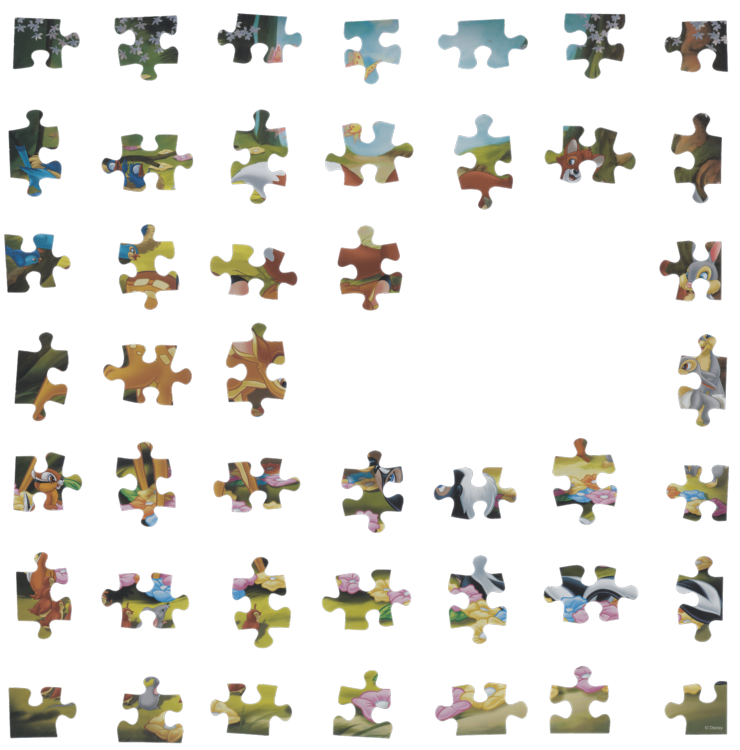
\includegraphics[width=0.6\textwidth]{images/puzzle_visualizer.png} 
\caption{Visualisierung eines Puzzle Zustands} 
\label{fig:solver_puzzle_visulizer} 
\end{figure}

\subsubsection[Simulated Annealing]{Simulated Annealing \myAuthor{Simon Hampp}}
\paragraph{Motivation}
Es wurde ein weiterer Ansatz gesucht, um unser Puzzle zu lösen, der eine alternative Vorgehensweise hat. Bisher wurden  klassische Verfahren entwickelt, wie den Depth Search Ansatz \autoref{sec:depth_search}. Zusätzlich wurde in der Vorlesung aber auch Simulated Annealing angesprochen, um das Puzzle zu lösen.

\paragraph{Simulated Annealing Allgemein}
Simulated Annealing ist ein Optimierungsverfahren. Der Hauptzweck ist es, globale Optima in komplexen, auch nicht differenzierbaren Landschaften zu finden, in denen viele lokale Optima vorhanden sein können. Simulated Annealing beginnt mit einer hohen "Temperatur", die es ermöglicht, große Änderungen zu akzeptieren, auch wenn diese die Lösungsqualität kurzfristig verschlechtern. Mit sinkender Temperatur werden solche "schlechten" Änderungen seltener angenommen, was der Suche hilft, sich auf eine bessere Lösungen zu konzentrieren.

\paragraph{Vorgehen}
Zu Beginn wurde Simulated Annealing unter Verwendung der Methoden existierender Bibliotheken von SciPy (scipy.optimize.basinhopping, scipy.optimize.minimize) ausprobiert, um das Annealing zu berechnen. Hierbei sind aber schnell Probleme aufgetreten, da das Puzzle Lösen Problem nicht differenzierbar ist und eine komplexe Optimierungsfunktion besitzt.

um das Puzzle zu lösen, wird eine Bibliothek benötigt, die nicht differenzierbare Funktionen erlaubt, und sich gut anpassen lässt. Während des annealing, müssen in unserem Fall bspw. mehrere Listen verwaltet werden, um zu vorherigen States zurückzukehren. Diese Anpassung wäre nicht oder nur schwer möglich, wenn  eine bestehende Methode von SciPy etc. benutzt wird.

\paragraph{Lösung}
Bei Simulated Annealing spielen zwei Funktionen eine zentrale Rolle. Die $move()$ Funktion, die einen Zustand ($state$) nimmt und daraus einen neuen Zustand generiert. Außerdem die $energy()$ Funktion, die die Güte eines Zustands berechnet. Beide Funktionen wurden für das Puzzle lösen implementiert. Als Basis für das tatsächliche annealing, wurde \textit{Simanneal} (https://github.com/perrygeo/simanneal) benutzt.

Da $simanneal.anneal()$ Listen als Funktionsparameter braucht und nicht zu viel bestehenden Code umgebaut werden sollte, aber das Puzzle ein $n \times n$ Array ist (mit $n = \#PuzzleTeile$), wird das Puzzle als $1 \times 2n^2$ dargestellt. Dabei stehen $n^2$ Positionen für das Puzzle und $n^2$ Positionen für die Rotationen zur Verfügung.

$$
[piece_0, rotation_0, piece_1, rotation_1, ... , piece_{n-1}, rotation_{n-1}]
$$

Um die Liste zurück auf das Array zu projektieren, wird die Position eines Puzzleteils in der Liste ganzzahlig halbiert und modulo die Seitenlänge genommen, so erhält man die Spalte des Teils im Puzzle Array. Um die Zeile zu erhalten, muss man die Position durch die Seitenlänge ganzzahlig teilen. \\
Bsp.: Puzzle $7 \times 7$ an Index $ 16 $ 

$$
Spalte = (16/2 \ modulo \ 7) = 1 
$$
$$
Zeile = (16/2) \ // \ 7 = 1
$$

In der $move()$ Funktion werden immer zwei zufällig Puzzleteile miteinander vertauscht und beide zufällig rotiert.

Die $energy()$ Funktion berechnet anhand der Liste und der Match Matrix, wie gut die Nachbarn jedes Puzzleteils zueinander passen, und summiert alle Matcher Werte auf. Damit diese Funktion effizienter wird, berechnet die Funktion nur die Energie neu, der vom letzten move betroffenen Puzzleteile. So wird die $energy()$ Funktion um mehrere Größenordnungen effizienter.

Mit dem Annealing konnte das $ 7 \times 7$ Puzzle nicht gelöst werden, die $energy()$ Funktion ist immer noch nicht effizient genug um den riesigen Parameterraum der Puzzles zu lösen. Da dem Annealer auch keine weitere Logik gegeben wird, als die Liste an Puzzle Positionen und Rotationen, probiert der Annealer "blind" aus.

\paragraph{Ausblick}
Damit das Annealing funktionieren könnte, müsste die $energy()$ Funktion noch effizienter werden. Außerdem könnte man noch mehr Nachbarschaftsinformationen berücksichtigen. Zum Beispiel sollten korrekte Nachbarschaften nicht mehr von der $move()$ Funktion aufgelöst werden. 



\subsubsection[Mock-Puzzle]{Mock-Puzzle \myAuthor{Luis Schubert}} \label{sec:mockpuzzle}
Zum Testen und Evaluieren der Solvingalgorithmen, unabhängig von anderen Komponenten des Praktikumsprojekts, simuliert das Mock-Puzzle ein Puzzle ohne dass dieses tatsächlich existieren und digitalisiert sein muss.

\paragraph{Motivation}
Da das Praktikumsprojekt in mehrere Teilprojekte unterteilt wurde gab es zu Beginn noch keine Matcher oder digitalisierten Puzzles um Solvingalgorithmen zu testen.
Um dieses Problem zu lösen lag eine Simulierung (Mocking) von Puzzles nahe.
Aufgrund des schnellen Fortschritts der Digitalisierung und des Matchings kam das Mock-Puzzle in dieser Hinsicht kaum zum Einsatz.
Zum Ende des Projekts zahlte es sich jedoch zur Evaluierung der Solvingalgorithmen aus, siehe Kapitel \ref{sec:evaluierung}.

\paragraph{Benötigte Funktionalität}
Um seinen Zweck der Simulation eines tatsächlichen Puzzles nachzukommen muss das Mock-Puzzle folgende Möglichkeiten bieten:
\begin{itemize}
    \item Simulieren von Puzzles beliebiger Größe
    \item Simulieren von Matchingergebnissen beliebiger Güte\\
        $\rightarrow$ Verrauschen der exakten Matchingergebnisse
    \item Schematische Visualisierung des simulierten Puzzles\\
        $\rightarrow$ Erstellen von Bildern der Puzzleteile
    \item Serialisierung von Puzzles zur reproduzierbarkeit von Tests

\end{itemize}

\paragraph{Implementierung}
Diese Anforderungen lassen sich durch vier zentrale Funktionalitäten realisieren:
\begin{itemize}
    \item Generierung eines gelösten Puzzles\\
        Hierzu wird über alle Positionen iteriert und je ein Puzzleteil mit zufälliger \verb|id| und Orientierung erstellt.
        Die Ecken (\verb|Male| / \verb|Female|) werden so gewählt, dass sie zu den bereits existierenden Puzzleteilen passen. Für Kanten, welche an keine bereits existierenden Puzzleteile angrenzen wird zufällig \verb|Male| oder \verb|Female| gewählt.
        Das Ergebnis ist das gelöste Puzzle, welches zur späteren Verwendung gespeichert wird. Pro erstelltem Puzzleteil wird ein Bild generiert, welches in Textform die \verb|id| des Puzzles, sowie dessen Kantentypen derstellt, siehe Abbildung \ref{fig:mock_puzzle}.
    \item "Mischen" des Puzzles\\
        Um einen realistischen, also gemischten Zustand zu simulieren werden die Puzzleteile anschließend um die zuvor zufällig bestimmte Orientierung zurückrotiert und nach aufsteigender \verb|id| sortiert.
    \item Erstellen der Matchmatrix\\
        Die Matchmatrix wird mithilfe der zuvor gespeicherten Lösung erstellt. Hierbei wird pro Kantenpaar überprüft, ob die entsprechenden Puzzleteile in der Lösung benachbart und so orientiert sind, dass siech das Kantenpaar berührt.
        Zum indirekten Zugriff auf die Inhalte der Matchmatrix implementiert die Klasse \verb|MockMatcher| das Matcherinterface.
    \item Verrauschen der Matchmatrix\\
        Da bisher nur perfekte Matchingergebnisse berechnet werden existiert die Option, alle Einträge der Matchmatrix zu verrauschen.

        Zur Berechnung des Eintrags $m_{i,j}$ an Stelle $i, j$ der Matchmatrix wird zunächst die Normalverteilung $\mathcal{N}$ berechnet und, falls nötig, an dessen Grenzen in den Bereich $[0, 1]$ gespiegelt:
        \begin{equation*}
            m_{i,j}' = 
            \begin{cases}
                \mathcal{N}(m_t, k_{noise}) & \texttt{ if } 0 \leq \mathcal{N}(m_t, k_{noise}) \leq 1 \\
                |\mathcal{N}(m_t, k_{noise})| & \texttt{ if } \mathcal{N}(m_t, k_{noise}) < 0 \\
                1 - \mathcal{N}(m_t, k_{noise}) + 1 & \texttt{ if } \mathcal{N}(m_t, k_{noise}) > 1
            \end{cases},
        \end{equation*}
        wobei $m_t \in \{0, 1\}$ das tatsächliche Matcherergebnis und $k_{noise}$ der Verauschungsgrad ist.
        Eine Begrenzung vom $m_{i,j}'$ auf den Bereich $[0, 1]$ ergibt anschließend $m_{i,j}$:
        \begin{equation*}
        m_{i, j} = 
            \begin{cases}
                m_{i,j}' & \texttt{ if } 0 \leq m_{i,j}' \leq 1 \\
                0 & \texttt{ if } m_{i,j}' < 0 \\
                1 & \texttt{ if } m_{i,j}' > 1
            \end{cases}.
        \end{equation*}
\end{itemize}

\begin{figure}[H] 
    \centering 
    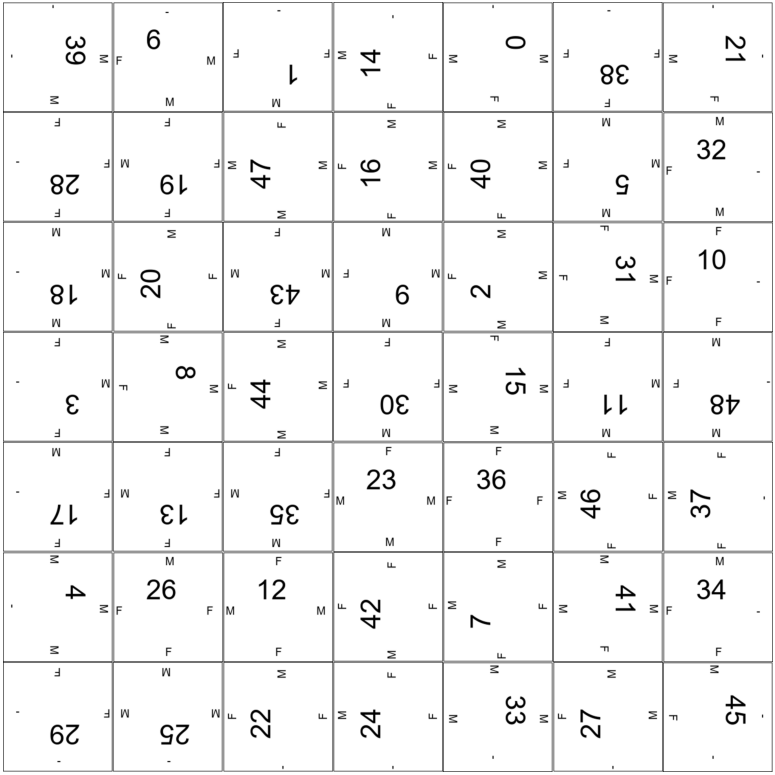
\includegraphics[width=0.7\textwidth]{images/mock_puzzle.png}
    \caption{Beispiel eines 7$\times$7 Mock-Puzzles.}
    \label{fig:mock_puzzle} 
\end{figure}


\subsubsection[Evaluierung]{Evaluierung \myAuthor{Luis Schubert}} \label{sec:evaluierung}
Im Folgenden werden die Erfolgsrate und Laufzeit der Solvingalgorithmen untersucht.

\paragraph{Ziel der Evaluierung}
Während eine Evaluierung anhand von realen Puzzles die aussagekräftigste ist, so ist ihre Durchführung für viele verschiedene Puzzlegrößen sehr aufwändig.
Um die Fähigkeiten der Solveralgorithmen angemessen zu evaluieren ist dies jedoch unabdinglich, da nur so die Grenzen der einzelnen Implementierungen erkundet werden können.

\paragraph{Durchführung}
Betrachtet sollen je Solveralgorithmus die Erfolgsquote beim Lösen verschiedener Puzzles und die dafür benötigte Zeit.
Hierzu werden Mock-Puzzles mit verschiedenen Dimensionen und Verrauschungsgraden jedem Solver zum Lösen übergeben und hierbei die Ausführungszeit gestoppt.
Um ein allgemeingültigeres Ergebnis zu erhalten wird dies, jeweils mit verschiedenen Puzzles, zehnmal durchgeführt.
Die Mock-Puzzles sind immer quadratisch, um eine einheitliche Darstellung zu ermöglichen.
Da alle Solvingalgorithmen einen Frame-Builder verwenden und bei einem quadratischen Puzzle die Anzahl der Puzzleteile im Rahmen minimal ist, sind quadratische Puzzles ohnehin eine sinnvolle Wahl zur Evaluierung.
Da der Annealing Solver das Lösen abbricht, sobald eine feste Zeit abgelaufen ist und nicht wie die anderen Solvingalgorithmen wenn seine Möglichkeiten ausgeschöpft sind, wird er in diesem Abschnitt nicht betrachtet.

\paragraph{Erfolgsquoten}
\begin{figure}[H] 
    \centering 
    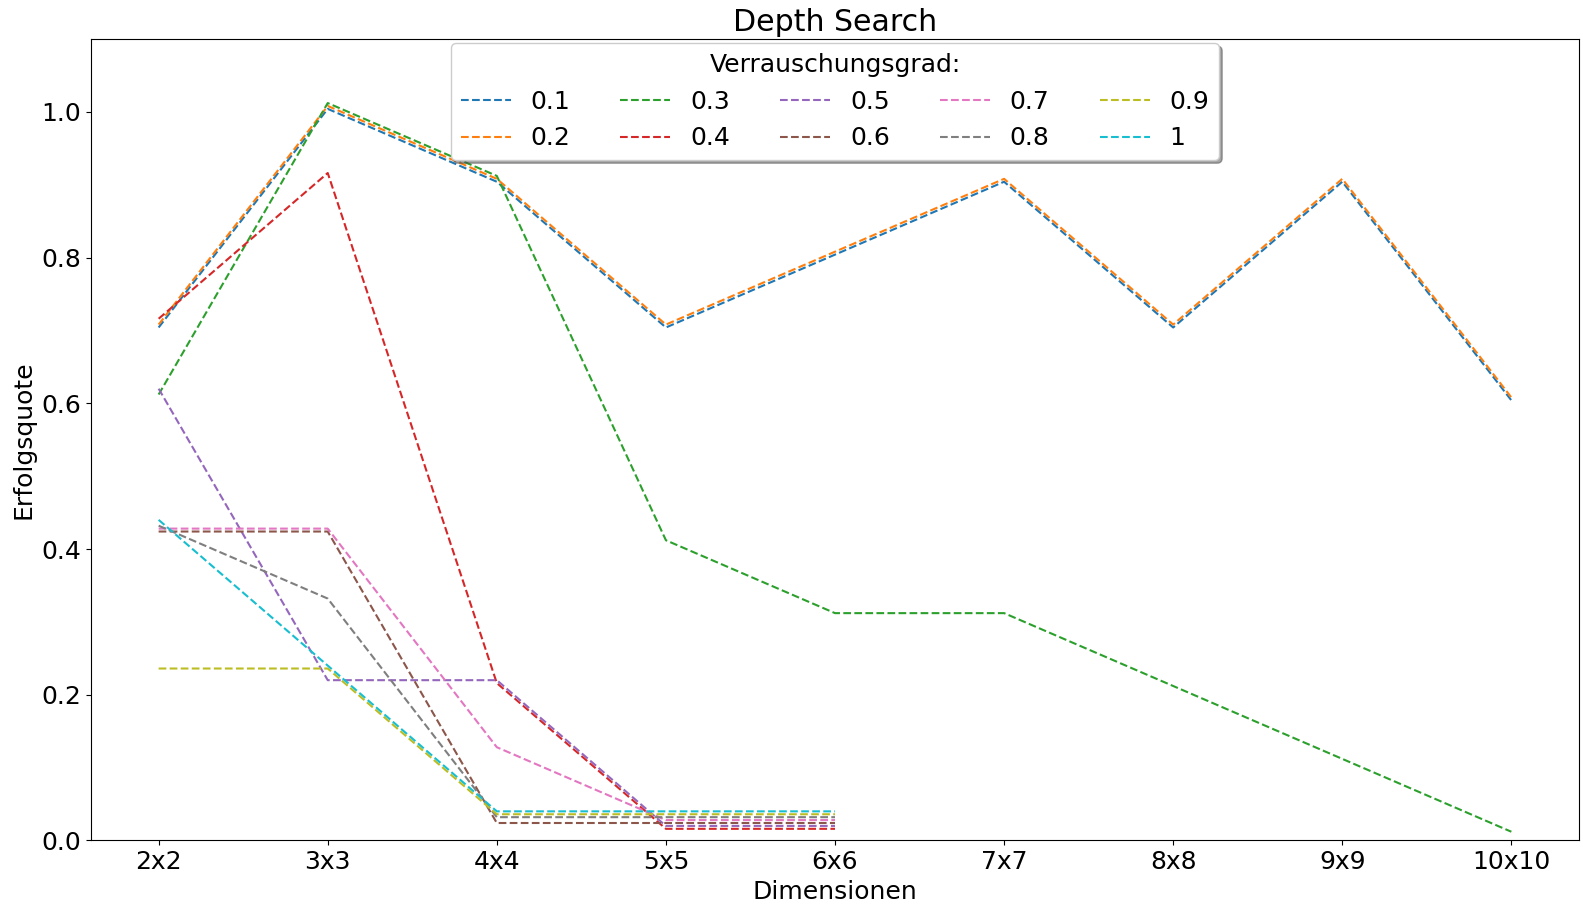
\includegraphics[width=\textwidth]{images/depth_search_eval.png}
    \caption{Evaluierungsergebnisse des Depth Search Solvingalgorithmus.}
    \label{fig:depth_search_eval} 
\end{figure}
Die Ergebnisse für Depth Seach, Easy First und Best First Solver verhalten sich ähnlich.
In Abbildung \ref{fig:depth_search_eval} ist zu erkennen, dass bei einem Verrauschungsgrad $k_{noise} \geq 0.4$ Puzzles mit einer Größe von über $3\times3$ kaum mehr gelöst werden können.
Bei $k_{noise} = 0.3$ können ab einer Größe über $7\times7$ nurnoch wenige Puzzles gelöst werden.
Anders verhält es sich für $k_{noise} \leq 0.2$. Damit werden auch bei Größen oberhalb von $7\times7$ noch über die Hälfte aller Puzzles gelöst.
Das ist insbesondere relevant, da die Accuracy eines Matchings für ein Mock-Puzzles mit $k_{noise} = 0.1$ immernoch unterhalb der von tatsächlichen Matchern (siehe Kapitel \ref{sec:matcher_evaluation}) liegt.
Ein Puzzle mit $k_{noise} = 0.1$ lässt sich also schwerer lösen als ein reales Puzzle, auf welches die implementierten Matcher angewandt werden.
Um nicht nur das best-case-Verhalten zu betrachten wird dieser Wert in den folgenden Evaluationen genutzt.

\paragraph{Laufzeiten}
\begin{figure}[H] 
    \centering 
    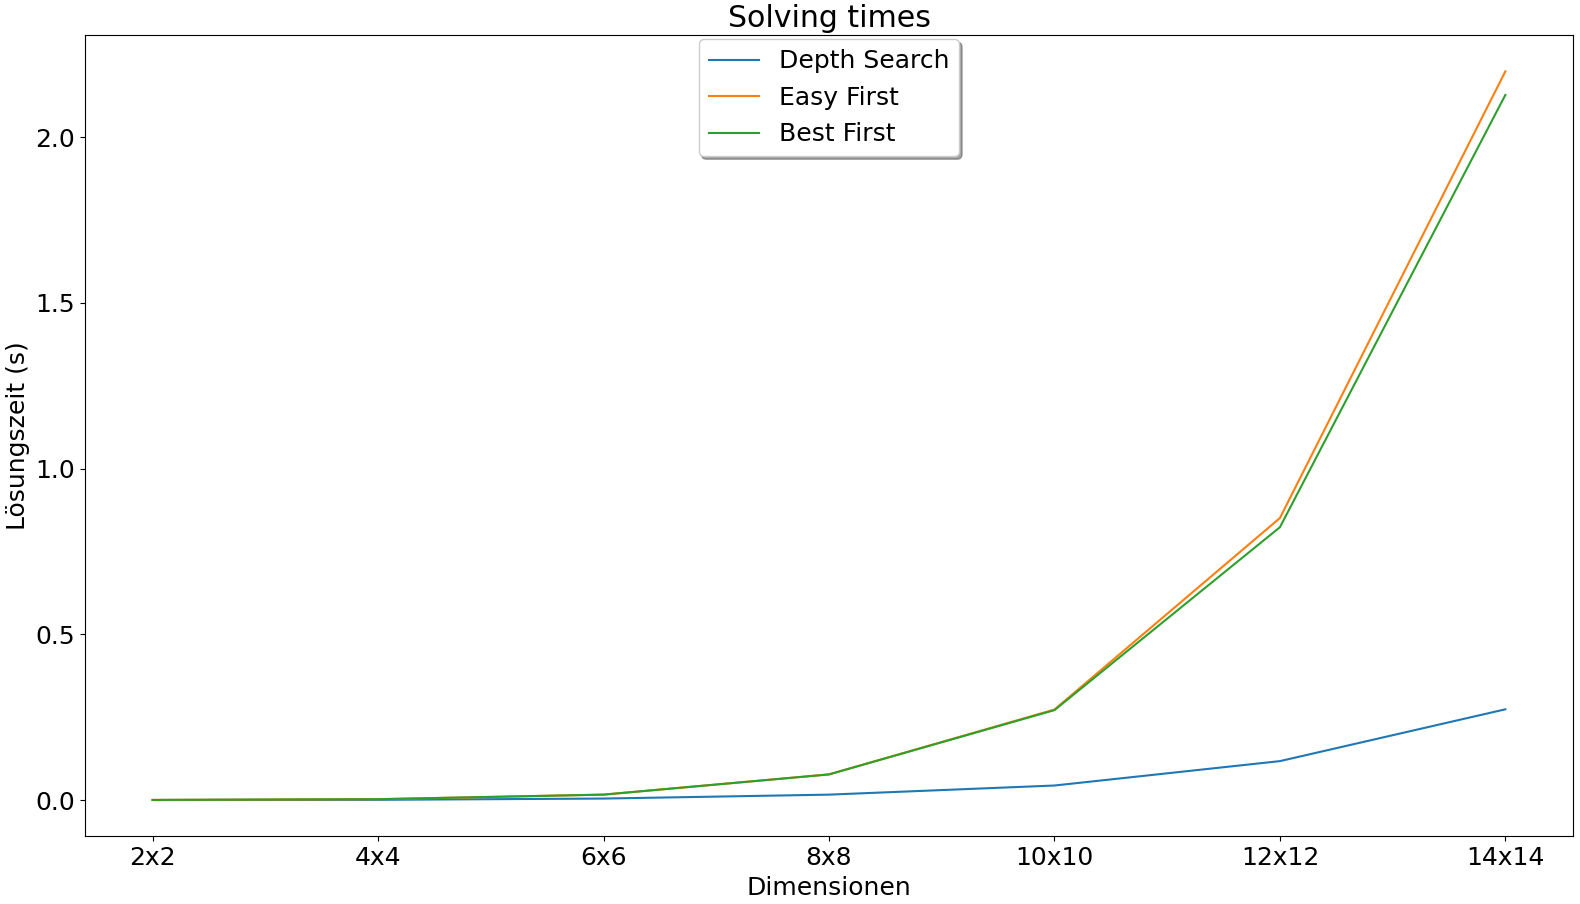
\includegraphics[width=0.8\textwidth]{images/all_solvers_time.png}
    \caption{Laufzeiten pro Lösungsdurchlauf.}
    \label{fig:all_solvers_time} 
\end{figure}
In Abbildung \ref{fig:all_solvers_time} lässt sich, wie zu erwarten, ein exponenzieller Anstieg in der Laufzeit bei zunehmender Puzzlegröße ablesen.
Da der Depth-first Solver hier am besten abschneidet während er in etwa die gleichen Erfolgsraten wie die anderen Solvingalgorithmen liefert wird nur zur Evaluierung größerer Puzzles betrachtet. 

\paragraph{Größere Puzzles}
\begin{figure}[H] 
    \centering 
    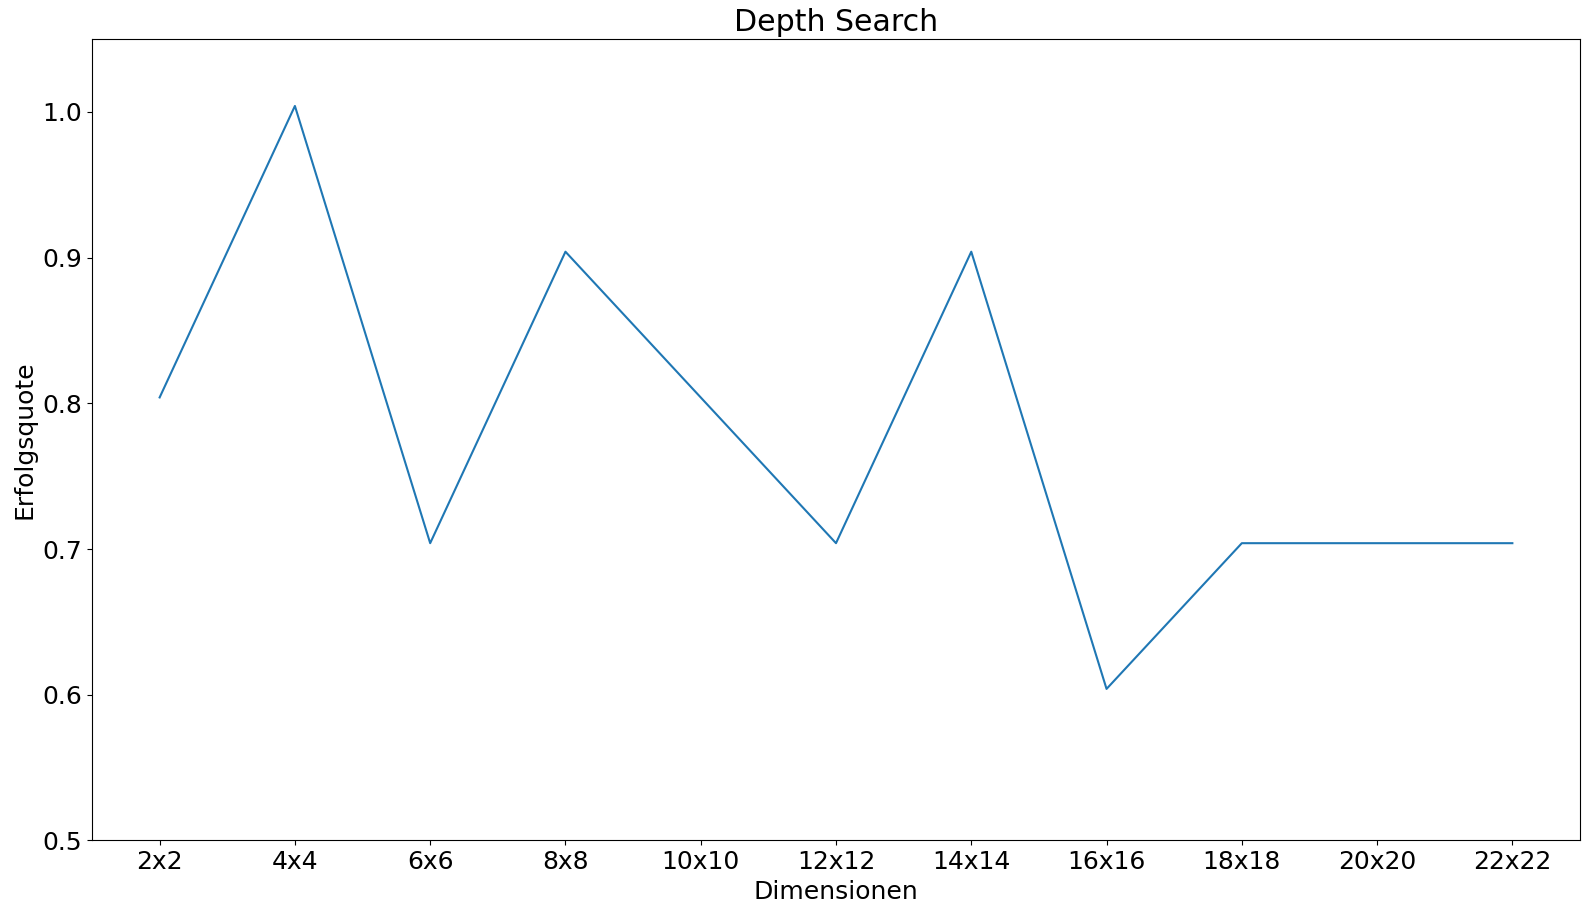
\includegraphics[width=0.8\textwidth]{images/eval_big_puzzles.png}
    \caption{Erfolgsquoten bei verschiedenen Puzzlegrößen.}
    \label{fig:eval_big_puzzles} 
\end{figure}
Wie in Abbildung \ref{fig:eval_big_puzzles} zu sehen ist, findet der Depth Search Solver auch bei Puzzlegrößen über $10\times10$ noch in den meisten Fällen die richtige Lösung. Eine zehnfache Evaluierung eines $22\times22$ Puzzles dauert etwa 37 Minuten.
